\chapter{Redox: Pathway Exploration}
\label{chap:redox}

\section{Purpose}
The purpose of this chapter is to describe Redox, a web application designed to run offline or deployed online, that is used to visualize, explore, and analyze large sets of biochemical network pathways.
Redox is currently still under active development by this author, with the scientists at Arzeda Inc (\url{http://arzeda.com/}) as the primary end users and source of feedback.
This chapter will present the motivation that lead to the development of this tool, the current design and features, and future directions of the application.
Redox uses Graphene extensively, and demonstrates the utility of Graphene as a tool for building data intensive, scientific web applications.

\section{Motivation}
\subsection{Metabolic engineering of microorganisms may yield new ways of producing valuable commodities}

Across the world, there is a desire to produce energy, fuel, and chemicals more efficiently and sustainably.
This has lead to the growth of industrial biotechnology, where microbes are used to convert organic raw materials into valuable commodities. \autocite{nielsen1998metabolic, sauer2012construction}
For example, from 2010 to 2012, bio-ethanol production increased from 10 billion liters to 75 billion liters.
Given these successes, biochemical industries are looking to move the production of additional chemical processes towards this direction.
While traditional fermentation techniques used naturally producing microorganisms, metabolic engineering today is focused on using a few select microbes as “platform cell factories” by applying genetic modifications.

\subsection{The space of candidate pathways is extremely large}
However, due to the complexity of cellular metabolism, this remains a significant challenge. \autocite{sohn2010genome}
Large numbers of interacting reactions combined with complex regulation make selecting candidate pathways for metabolic engineering difficult.
For example, within the KEGG Database alone, there are nearly 10,000 biochemical reactions and over 17,000 metabolites and small molecules cataloged.

\subsection{Semi-automated pathway selection requires user curation}
Arzeda is a synthetic biology company that approaches this problem using a unique computational design technology that can narrow down the space of potential reaction pathways.
However, it still remains a challenge for scientists to pick a handful pathways to examine more closely and bring in to the lab from the pool of candidate pathways.


\section{Solution}

\subsection{Iterative sorting, filtering, and pinning to hone in on desired output}

The Redox approach to obtaining meaningful results from a possibly overwhelming set of solutions is through iterative data filtering and visualization (Figure~\ref{Figure:redox-flow}).

The initial step involves loading the data set that contains all definitions for all candidate pathways.
Each pathway contains definitions for the reactions involved, and each reaction contains definitions for the chemical species involved.
Redox first looks for this file in a specific directory on the web server, but it may also be loaded through the client after the application has started.

The starting point for the user is the table view (Figure~\ref{Figure:redox-table-view}).
Here the users can sort and filter pathways by various characteristics, such as number and types of intermediates involved.
Pathways of interest may then be pinned, which adds the pathway to the sidebar and automatically assigns a color code (Figure~\ref{Figure:redox-table-pinned}).

\begin{wrapfigure}{i}{0.35\textwidth}
  \includegraphics[width=0.3\textwidth, page=29,trim=0cm 0cm 18.3cm 0cm, clip=true]{images/Figures.pdf}
  \caption{Redox is designed for iterative sorting, filtering, and analysis. The user provides an input data file, which is parsed into a sortable table. Interesting pathways may be pinned and then visualized, before exporting the final selection of pathways.}
  \label{Figure:redox-flow}
\end{wrapfigure}
\subsection{Visualize candidate pathways}

Selected pathways can then be further inspected in the graph view (Figure~\ref{Figure:redox-graph-highlight}).
All compounds involved in the selected pathways are represented as nodes in the graph, and edges are drawn between nodes based on the all reactions within the pathway.

In order to see which compounds and reactions belong to a particular pathway, the user may hover over the pathways in the sidebar to highlight individual pathways (Figures~\ref{Figure:redox-graph-highlight1}-\ref{Figure:redox-graph-highlight2}).
On mouse hover a node, a popup will open to display details about the node (Figure~\ref{Figure:redox-detail-hover}), such as its molecular structure and an external link to compound profile page in the ChEBI database (Figure~\ref{Figure:redox-detail-chebi}).

The network diagram is customizable and interactive.
Nodes may be dragged and pinned, and the layout settings panel in the sidebar allows different properties of the force layout to be modified (Figure~\ref{Figure:redox-template-a}).
Since Graphene allows for the layout view to be defined independently of the model data, the view template may be switched on-the-fly (Figure~\ref{Figure:redox-template-b}).
One possible usage of this feature would be to display nodes as small shapes during the data reduction process, and then switching to a detailed view where each node is represented by the molecular structure of the underlying compound.

\subsection{Export curated selection of pathways}

After adding all desired and removing all undesired pathways, the user may then export (through the export tab) the collection in a standard JSON format, which is a subset of the original input data.
It is also possible for the results of a particular session to be used as the starting data set for the next Redox session.

\section{Implementation}

\subsection{Table View}
When a new data set is added, it is parsed into separate arrays containing compounds, reactions, and pathways.
Lookup hash tables are also used to quickly find elements by ID, rather than using less efficient searches through the array.

The table view template is then as follows:

\begin{lstlisting}[language=html]
<!-- Loop through array of pathways, starting at the first item on the page, stopping at the page size-->
<tr ng-repeat="pathway in reactionSets | startFrom:page.current*page.size | limitTo:page.size">
  <td>
    <!-- show the pathway ID -->
    {{pathway['@id']}}
  </td>
  <td>
    <!-- show the number of intermediates of pathway -->
    {{pathway.set.length}}
  </td>
  <td>
    <!-- Add the ID to the pinned set on click -->
    <button class="btn btn-default" ng-click="clickPin(set['@id'])">
      <span class="fa-stack">
            <!-- show checkmark if the pathway is pinned -->
            <i class="fa fa-square-o fa-stack-2x"></i>
            <i ng-if="_.contains(display.pinned, set['@id'])" class="fa fa-check fa-stack-1x"></i>
          </span>
    </button>
  </td>
</tr>
\end{lstlisting}

The view also includes the filter functions \texttt{startFrom} and \texttt{limitTo}. Additional filter functions will be added to further customize sorting.

\subsection{Graph View}
The Graph view also shares the same underlying data model as the Table view, including helper data structures, such as the \texttt{display} hash that keeps track of information related to the application state.
The data controller attached to the graph observes the pinned pathway set.
Changes in the pinned pathway set trigger a redefinition of the graph nodes and edges, and invoke the D3 force layout algorithm for node placement.

A mouseover function is attached to the sidebar list of pinned sets, which switched the currently highlighted set ID as the one underneath the mouse cursor.
A watcher function observes changes in the highlighted set ID and upon change loops through the graph nodes to highlight the elements related to the pathway.
The below is an example of this watcher function:
\begin{lstlisting}[language=JavaScript]
var reactionSet = _.find($scope.reactionSets, {
  '@id': newVal // newVal is the newly selected pathway
});
_.each($scope.nodes, function (n) {
  if (_.contains(reactionSet.set, n.id) // first check if the node ID matches the reactions listed
      || _.intersection(_.keys(n.reactions), reactionSet.set).length // each node contains a hash table with reactions that the compound is a part of
     ) {
    n.color = $scope.colors(index); // the set index is used to lookup the color value
  } else {
    n.color = 'whitesmoke';
  }
});
\end{lstlisting}

\subsection{Swappable layout templates}
Changing templates is supported by Graphene, and thus Redox simply needs to pass in a reference to the template name, which may be changed through user input.

\begin{lstlisting}[language=html]
<sg-graphene imports="exports" template="views/{{selected.template}}.html"></sg-graphene>
\end{lstlisting}

\section{Future Directions}
Redox is currently still under heavy development.
Its core functionality and design goals have been presented in this chapter.
Additional features that will be added to Redox are: enhanced sorting through additional filters, as mentioned previously, additional templates for more visualization options, and the ability automatically handle node aliasing for highly connected graphs which are detrimental to the overall layout.
Feedback from the Arzeda users will also be incorporated into future designs.


\begin{figure}
  \centering
  \begin{subfigure}[b]{\textwidth}
    \includegraphics[width=\textwidth, page=5,trim=0.37cm 3.65cm 13.1cm 3.3cm, clip=true]{images/Figures.pdf}
    \caption{The table view lists all pathways in a paginated format.
      The user can browse the tabulated pathways and sort by metadata.}
    \label{Figure:redox-table-view}
  \end{subfigure}
  \begin{subfigure}[b]{\textwidth}
    \includegraphics[width=\textwidth, page=5,trim=13.1cm 3.65cm 0.37cm 3.3cm, clip=true]{images/Figures.pdf}
    \caption{Pinned pathways are added to the sidebar and encoded with a color from palette.}
    \label{Figure:redox-table-pinned}
  \end{subfigure}
  \caption{The Redox Table View allows users to parse through numerous pathways and select individual candidates for further examination.}
  \label{Figure:redox-table}
\end{figure}

\begin{figure}
  \centering
  \begin{subfigure}[b]{\textwidth}
    \includegraphics[width=\textwidth, page=6,trim=0.37cm 3.65cm 13.1cm 3.3cm, clip=true]{images/Figures.pdf}
    \caption{Mouse hover over the pathway list color codes all the related reactions and species involved in the pathway. In this template, circles indicate species and squares denote reactions.}
    \label{Figure:redox-graph-highlight1}
  \end{subfigure}
  \begin{subfigure}[b]{\textwidth}
    \includegraphics[width=\textwidth, page=6,trim=13.1cm 3.65cm 0.37cm 3.3cm, clip=true]{images/Figures.pdf}
    \caption{Hovering over the next list item will quickly switch the color coding, allowing the user to explore the pathways.}
    \label{Figure:redox-graph-highlight2}
  \end{subfigure}
  \caption{Redox Graph creates a connected network diagram from all selected pathways.}
  \label{Figure:redox-graph-highlight}
\end{figure}

\begin{figure}
  \centering
  \begin{subfigure}[b]{\textwidth}
    \includegraphics[width=\textwidth, page=8,trim=0.37cm 3.65cm 13.1cm 3.3cm, clip=true]{images/Figures.pdf}
    \caption{Upon node hover, a pop-up window shows the relevant chemical structure of the species of reaction diagram.
      The sidebar also populates with a link to the ChEBI web page.}
    \label{Figure:redox-detail-hover}
  \end{subfigure}
  \begin{subfigure}[b]{\textwidth}
    \includegraphics[width=\textwidth, page=8,trim=13.1cm 3.65cm 0.37cm 3.3cm, clip=true]{images/Figures.pdf}
    \caption{Clicking on the link to ChEBI leads directly to the species information page.}
    \label{Figure:redox-detail-chebi}
  \end{subfigure}
  \caption{Exploring graph details.}
  \label{Figure:redox-detail}
\end{figure}

\begin{figure}
  \centering
  \begin{subfigure}[b]{\textwidth}
    \includegraphics[width=\textwidth, page=7,trim=0.37cm 3.65cm 13.1cm 3.3cm, clip=true]{images/Figures.pdf}
    \caption{In the sidebar, sliders allow the user to interactively change force directed layout settings, such particle charge and gravity.}
    \label{Figure:redox-template-a}
  \end{subfigure}
  \begin{subfigure}[b]{\textwidth}
    \includegraphics[width=\textwidth, page=7,trim=13.1cm 3.65cm 0.37cm 3.3cm, clip=true]{images/Figures.pdf}
    \caption{Graphene templates may be swapped out on the fly to change the graph.
      Due to the separation of model and view, the underlying data is unchanged when the view is switched.}
    \label{Figure:redox-template-b}
  \end{subfigure}
  \caption{The Redox layout is highly customizable.}
  \label{Figure:redox-template}
\end{figure}


